\section{Results and Discussion}
\label{sec:results}

We evaluated the performance of EDEN on a series of benchmark functions to assess its effectiveness on optimization problems of varying complexity. Initially, we verified the correctness of the method using the Sphere, a simple unimodal function. Subsequently, we tested EDEN on more challenging multimodal functions, including the Rastrigin, Ackley, and Griewank functions, all within a 100-dimensional search space.


The method performances were compared against a standard Genetic Algorithm (GA) \cite{holland_ga_1992} and the Covariance Matrix Adaptation Evolution Strategy (CMA-ES) algorithm \cite{hansen_cma_2001}. All methods where compared over 10,000 fitness evaluations and the results are shown in Table \ref{tab:results} and Figures \ref{fig:sphere}, \ref{fig:rastrigin}.

\begin{table}[H]
    \centering
    \caption{Best fitness found by each algorithm on the benchmark functions}
    \begin{tabular}{|c|c|c|c|}
        \hline
        Function  & EDEN     & GA       & CMA-ES    \\
        \hline
        Sphere    & 1.049    & 85.972   & 7.931e-14 \\
        Rastrigin & 251.234  & 1010.571 & 57.073    \\
        Ackley    & 4.981e-3 & 4.953    & 3.532e-7  \\
        Griewank  & 5.974    & 435.020  & 3.731e-6  \\
        \hline
    \end{tabular}
    \label{tab:results}
\end{table}

\begin{figure}
    \centering
    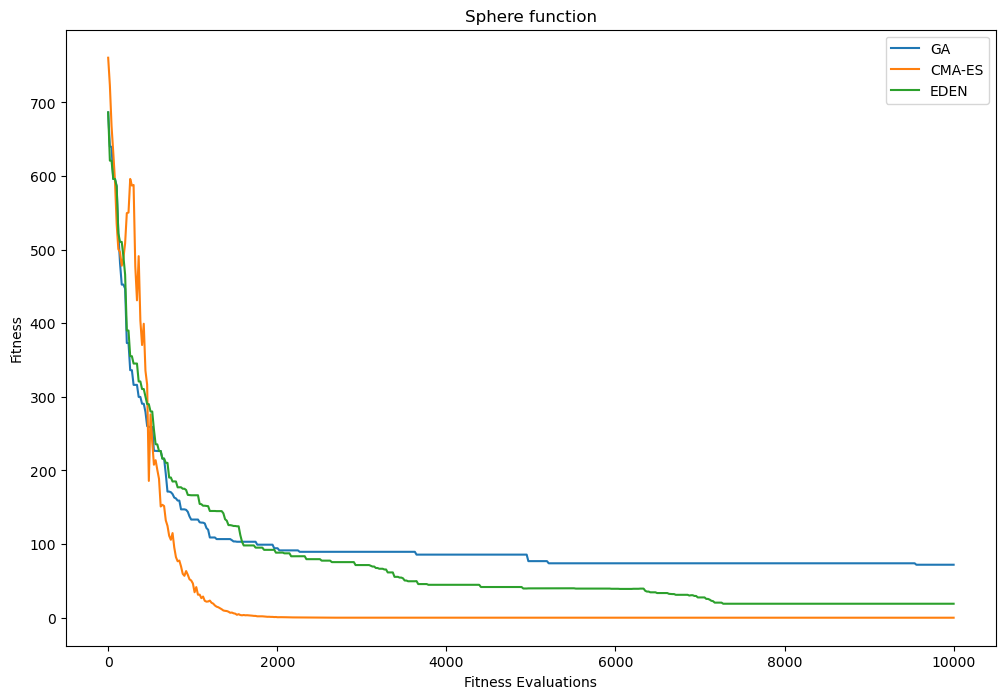
\includegraphics[width=0.4\textwidth]{img/sphere.png}
    \caption{Comparison on the Sphere function}
    \label{fig:sphere}
\end{figure}

\begin{figure}
    \centering
    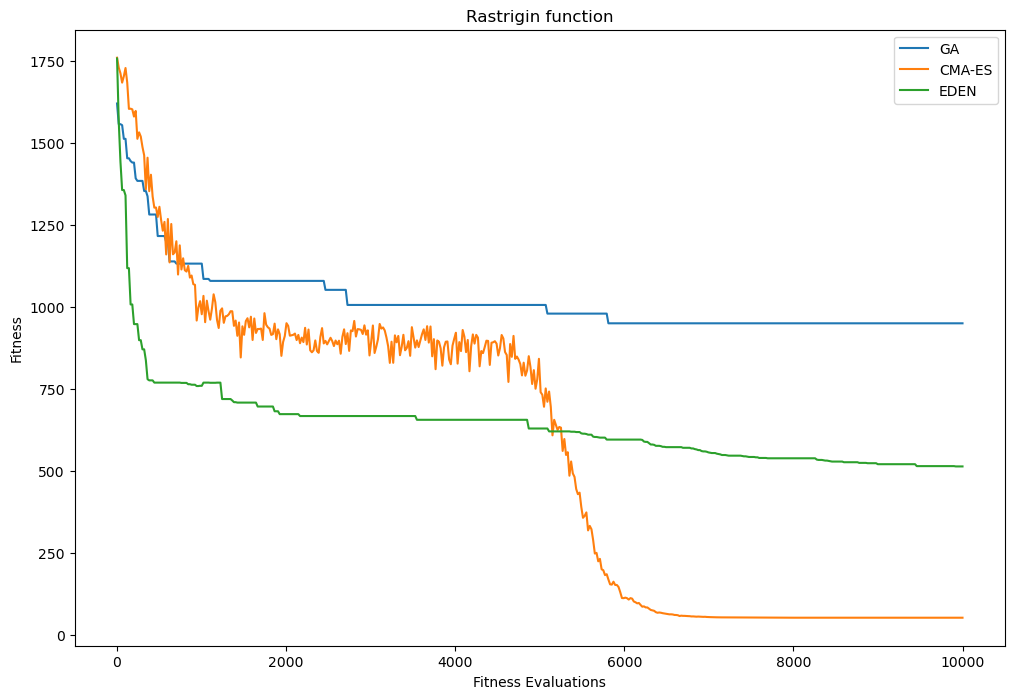
\includegraphics[width=0.4\textwidth]{img/rastrigin.png}
    \caption{Comparison on the Rastrigin function}
    \label{fig:rastrigin}
\end{figure}

The results indicate that CMA-ES consistently outperforms the other algorithms across all benchmarks. While EDEN surpasses the GA in all cases, it still lags behind CMA-ES. Interestingly, EDEN struggled more with the Sphere function than expected, despite its relative simplicity.

The poor performances of EDEN are likely not due to the fitting abilities of the model itself, but a consequence of the sampling method. Langevin dynamics performance is heavily dependent of the choice of the learning rate and the noise parameter. Even with an adaptive noise parameter to help focusing the sampling on increasingly smaller areas, we found the method still struggles to focus on a specific region thus hindering the convergence to the global optimum.

% \subsection{Possible Improvements}
% Testing the method on deceptive benchmark functions, such as the trap function, could provide deeper insights into its ability to exploit epistasis. For instance, MOA \cite{shakya_moa_2011} uses the binary trap5 function as a deceptive benchmark:
% \begin{align*}
%     f_{trap,k}(x) = \sum_{i=1}^{n/k}trap_{k}(x_{b_i,1} + \ldots + x_{b_i,k}) \\
%     trap_{k}(u) = \begin{cases}
%                       f_{high}                          & \text{if } u = k \\
%                       f_{low}   - u \frac{f_{low}}{k-1} & \text{otherwise}
%                   \end{cases}
% \end{align*}
% where $u$ is the number of ones in the input block of $k$ bits, and $f_{high}$ and $f_{low}$ are parameters that control the distance between the local and global optima.

% Additionally, expanding the analysis to include comparisons with other EDA algorithms would provide valuable insights into EDEN’s relative performance and identify potential areas for improvement.
